\section{Durchführung}

Eine Phasenregelschleife besteht aus drei Funktionsblöcken (\ref{fig:Blockschaltbild_PLL}), die in dem Versuch hintereinander aufgebaut werden.

\begin{figure}[H]

  \centering
{

\tikzstyle{block} = [draw, rectangle, minimum height=3em, minimum width=6em]
\tikzstyle{input} = [coordinate]
\tikzstyle{output} = [coordinate]
\tikzstyle{knot} = [postaction={decorate}, decoration={markings,mark=at position 0 with {\fill circle [radius=2pt];}}]

\begin{tikzpicture}[auto, node distance=3.5cm,>=latex']
    % Define nodes
    \node [input, name=input] {};
    \node [block, right of=input] (block1) {Referenzsignal};
    \node [block, right of=block1] (block2) {Phasendetektor};
    \node [block, right of=block2] (block3) {Schleifenfilter};
    \node [block, right of=block3] (block4) {VCO};
    \node [output, right of=block4] (output) {};

    % Connect the nodes
    %\draw [->] (input) --   (block1);
    \draw [->] (block1) -- node {$U_{\mathrm{ref}}$} (block2);
    \draw [->] (block2) -- node {$U_{pd}$} (block3);
    \draw [->] (block3) -- node {$U_{f}$}(block4);
    \draw [->] (block4) -- node {$U_{\mathrm{out}}$} (output);
     \draw [knot,->] ($(output)-(1,0)$)  |- ++(0,-1.5) -| (block2.south) node[near start,below] {Feedback};
\end{tikzpicture}
}
\caption{Blockschaltbild PLL}
\label{fig:Blockschaltbild_PLL}
\end{figure}

Im Folgenden werden der Aufbau des VCOs, des Phasendetektors und des Schleifenfilters näher erläutert. Abschließend erfolgt die Erklärung des Zusammenbaus.

\subsection{Dreieck-Rechteck-VCO}

In diesem Teilversuch wurde ein Dreieck-Rechteck-VCO \ref{fig:VCO_circuit} aufgebaut.
Es wurden folgende Bauteile verwendet:
%
\begin{itemize}
    \item ohmsche Widerstände $R_1$=\SI{18}{\kilo\ohm}, $R_2$=\SI{27}{\kilo\ohm}, $R_3$=\SI{820}{\ohm}, $R_4$=\SI{460}{\ohm}, $R_5$=$R_6$=\SI{1,2}{\kilo\ohm}
    \item Kondensator $C_1$=\SI{100}{\nano\farad}
    \item Operationsverstärker TL074
    \item 1x NPN-Transistor, 1x PNP-Transistor
\end{itemize}

Die Abbildung \ref{fig:VCO_circuit} zeigt die Anordnung jeweiliger verwendeten Bauteile der VCO auf dem Steckbrett.

\begin{figure}[H]
  \centering
  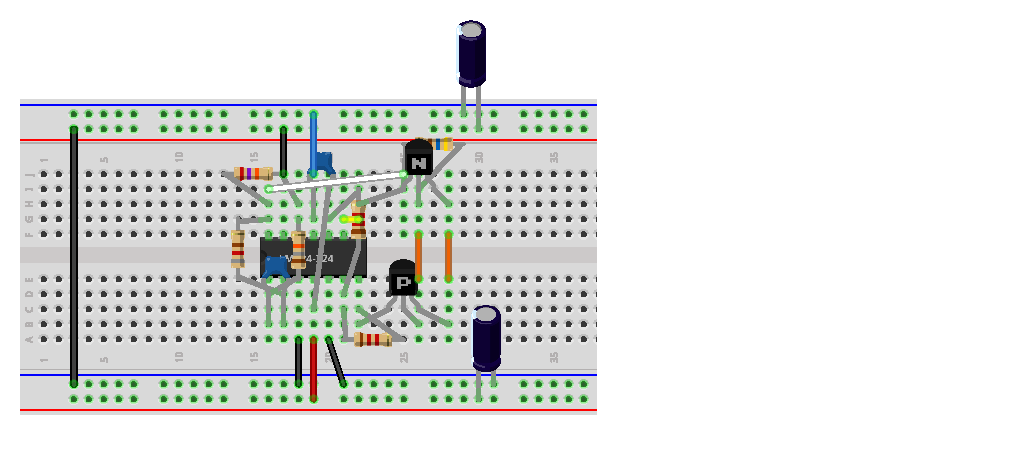
\includegraphics[width=0.6\linewidth]{Elektronik-Laborprotokoll_PLL/circuits/VCO_circuit.pdf}
  \caption{VCO (Steckbrett)}
  \label{fig:VCO_circuit}
\end{figure}



\subsection{Phasendetektor}


In diesem Teilversuch wird ein digitaler Phasendetektor aufgebaut.
Es werden folgende Bauteile verwendet:
%
\begin{itemize}
    \item ohmsche Widerstände $R_7$=$R_8$=$R_9$=$R_{10}$=\SI{1}{\kilo\ohm}
    \item Operationsverstärker TL072
    \item 1 x AND-Gatter
    \item 2x D-Flip-Flops
\end{itemize}

\subsection{Schleifenfilter}

In diesem Teilversuch wird als Schleifenfilter ein PI-Filter aufgebaut.
Es werden folgende Bauteile verwendet:

\begin{itemize}
    \item ohmsche Widerstände $R_{11}$=\SI{39}{\kilo\ohm}, $R{12}$=\SI{12}{\kilo\ohm}
    \item  Kondensator $C_2$=\SI{1}{\micro\farad}
    \item Operationsverstärker TL072
\end{itemize}

Die Abbildung \ref{fig:Pd_und_PI_circuit} darstellt, wie der Phasendetektor und das Schleifenfilter auf dem Steckbrett aufgebaut werden.

\begin{figure}[H]
  \centering
  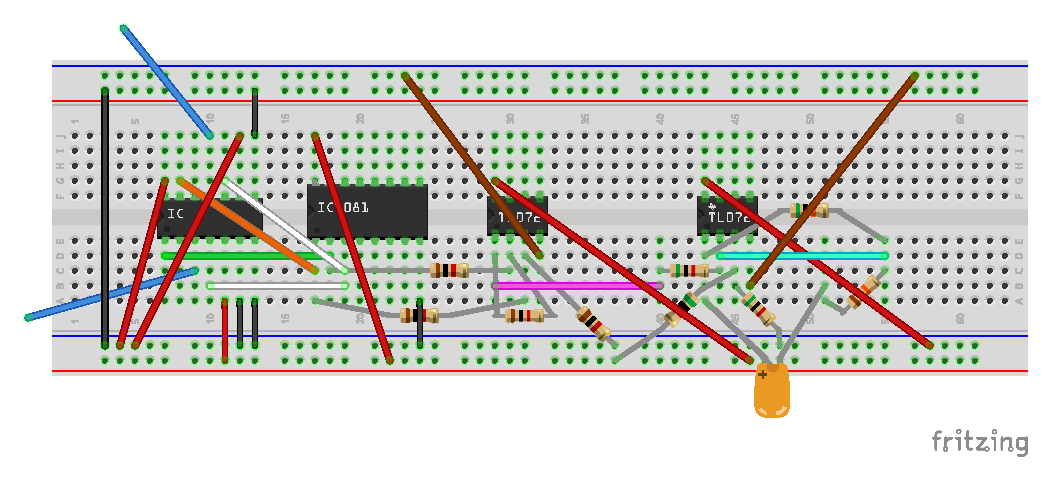
\includegraphics[width=0.8\linewidth]{Elektronik-Laborprotokoll_PLL/circuits/Phasendetektor_und_Filter_circuit.pdf}
  \caption{Phasendetektor und Schleifenfilter (Steckbrett)}
  \label{fig:Pd_und_PI_circuit}
\end{figure}

\subsection{Die Teile der PLL zusammenbauen}

Nachdem jeder der drei Funktionsblöcken einzeln aufgebaut wurden, werden diese Teile unter Verwendung einiger Widerstände und Dioden zusammengebaut. Dafür werden folgende Bauteile benötigt:

\begin{itemize}
    \item ohmsche Widerstände $R_{13}$=\SI{100}{\kilo\ohm}, $R_{14}$=\SI{1,5}{\kilo\ohm}
    \item  2 x Dioden
\end{itemize}

Wie in der Abbildung \ref{fig:PLL_zusammengebaut} zu sehen ist, wird der Ausgang des Phasendetektors direkt mit dem Eingang des PI-Filters verbunden. Der Ausgang des Schleifenfilters wird über einer Diode $D1$,deren Kathode über einen hochohmigen Widerstand $R_{13}$ an die Masse verbunden ist, mit dem Eingang der VCO verbunden. Der Ausgang der VCO wird über einen Widerstand $R_{14}$, der über einen Diode $D2$ mit dem Eingang des Phasendetektors verbunden. An dem anderen Eingang des Phasendetektors befindet sich ein Referenzsignal.

%HALLO JUAN WELCOME

\begin{figure}[H]
  \centering
  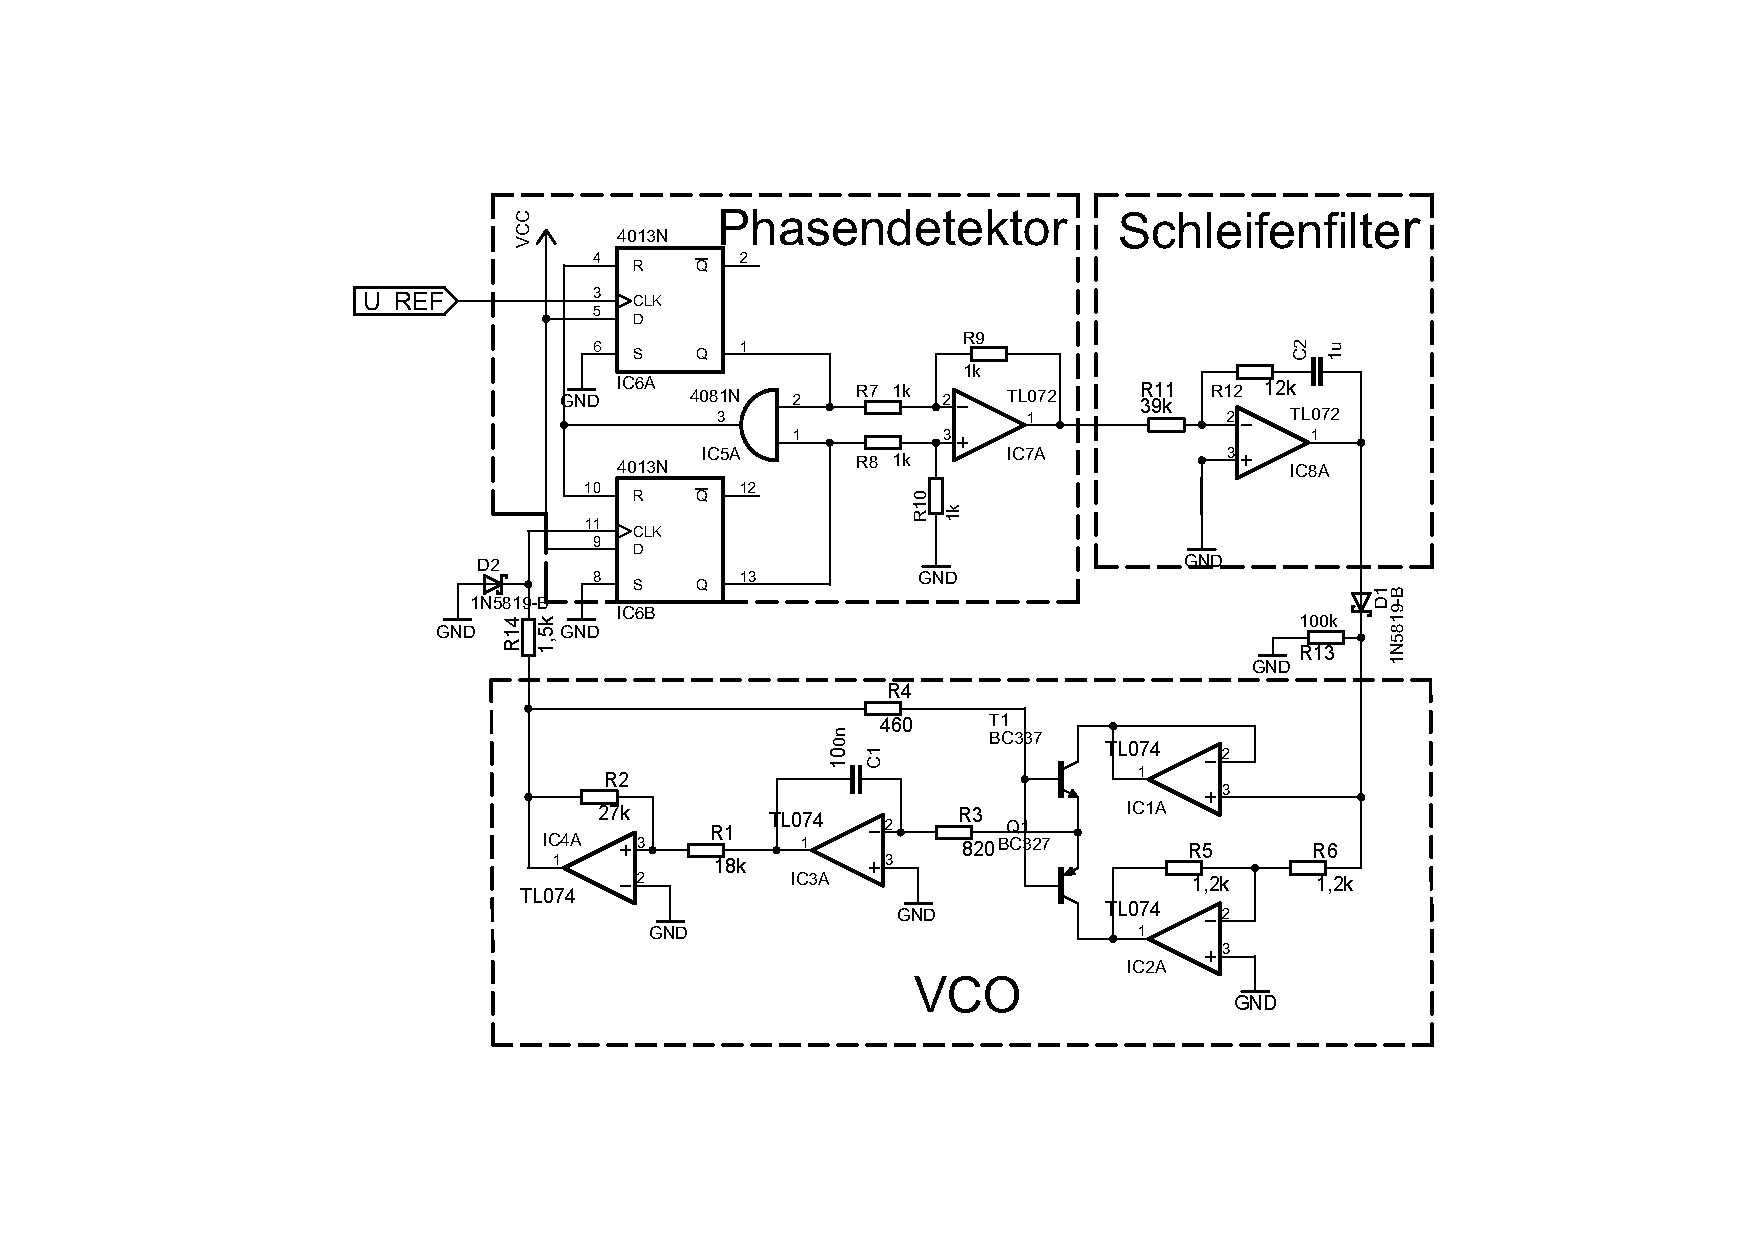
\includegraphics[width=1\linewidth]{Elektronik-Laborprotokoll_PLL/Abbildungen/PLL_Schaltung_zusammengebaut.pdf}
  \caption{PLL zusammengebaut (Abbildung geändert nach dem Beispielentwurf \cite{SkriptElektronik})}
  \label{fig:PLL_zusammengebaut}
\end{figure}


